\chapter{Turing Machine Obfuscator}

%
\section{Design Overview}
In a program, a branch condition statement compares two operands and selects a
branch for control transfer based on the comparison result. As aforementioned,
Turing machine has been proved to be able to simulate the semantics of any
functional component of a program. Hence, any program branch condition statement
can be modeled by a Turing machine. Taking advantage of its powerful computation
ability as well as execution complexity, we propose to employ Turing machine to
obfuscate branch condition statements (the branch condition statement is
referred as ``branch predicate'' later in this thesis since its output is usually
a boolean value) in a program. A Turing machine obfuscated branch condition
statement is shown in \F~\ref{fig:two}. Instead of directly computing a boolean
value through a comparison instruction, we feed a Turing machine with the inputs
(the value of operands) and let the Turing machine to simulate the comparison
semantics.

\begin{figure}
 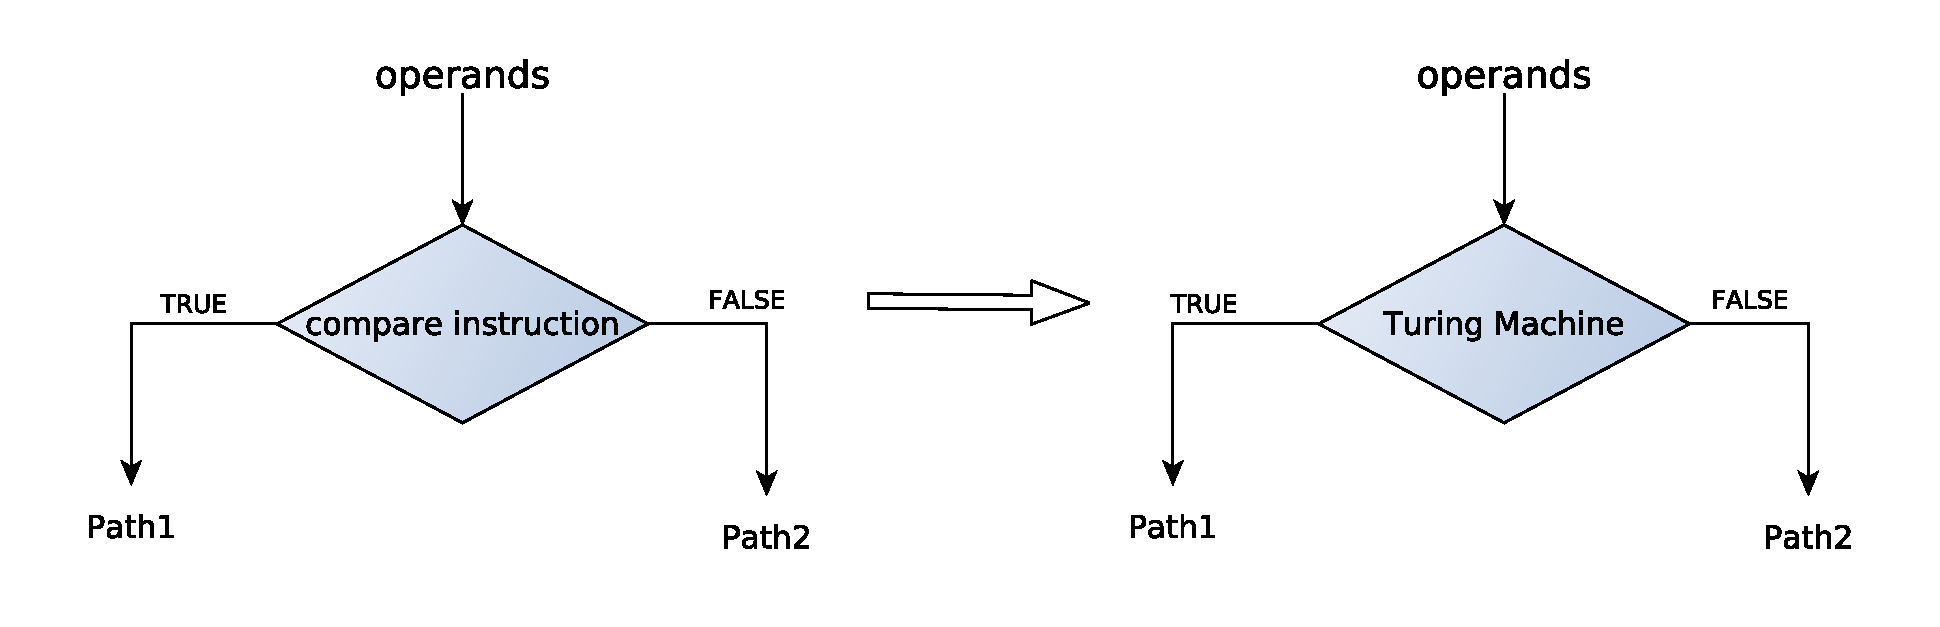
\includegraphics[width=\linewidth]{figure2.eps}
 \caption{Obfuscate a branch condition statement through a Turing machine.}
 \label{fig:two}
\end{figure}

\section{Turing Machine}
As shown in \F~\ref{fig:three}, a typical Turing machine consists of four
components:
\begin{itemize}
  \item An infinite-long tape which contains a sequence of cells. Each cell
    holds a symbol defined in the tape alphabet (the alphabet is introduced
    shortly). In this work, our proposed Turing machine obfuscator would
    dynamically allocate new tape cells to construct an infinite tape to store
    intermediate results.
  \item A tape head which could perform \texttt{read}, \texttt{write},
    \texttt{move left} and \texttt{move right} operations over the tape.
  \item A state register used to record the state of the Turing machine. Turing
    machine states are finite and defined in the transition table.
  \item A transition table that consists of all the transition rules defining
    how a Turing machine transfers from one state to another.
\end{itemize}

Although simple, Turing machine model resembles a modern computer in several
ways. The head is I/O device. The infinite tape acts as the computer memory. The
transition table defines the mission of this Turing machine which is like the
program code and data. Hence, Turing machine is also deemed as the foundation of
modern computer science development.

\begin{figure}
 \includegraphics[width=0.9\linewidth]{TM.pdf}
 \caption{Turing machine components.}
 \label{fig:three}
\end{figure}

\subsection{Transition Table}
A transition rule could be represented by a five-element tuple $(S_c, T_c, S_n,
T_n, D)$ where:

\begin{itemize}
  \item \(S_c\) is the current Turing machine state
  \item \(T_c\) is the current tape cell symbol read by the head
  \item \(S_n\) is the new Turing machine state
  \item \(T_n\) is the symbol head writes to the current tape cell
  \item \(D\) is the direction the head should move (i.e., ``left'' or
    ``right'')
\end{itemize}

In general, every five-element tuple represents a transition table rule shown in
\F~\ref{fig:three}.

\subsection{Turing Machine Encoding}
Initially, Turing machine is at the ``start'' (\(S_0\)) state and tape records
the Turing machine input. Consistent with existing Turing machine simulator
project~\cite{SingleTape}, blank symbol is denoted as ``*'' on the tape, while
the length of ``$\cdot$'' is used to encode an operand of integer type (our
current implementation only focuses on operand of integer type, we present
further discussion on this in \S\ref{subsec:phase-three}). For instance, integer
5 is represented as five continuous ``$\cdot$'' on the tape. Note that a Turing
machine could be encoded with various of ways, our prototype represents only one
of them. Turing machine with different encoding strategies operates with totally
distinct execution pattern. This also makes Turing machine obfuscation hard to
be analyzed.

In general, our Turing machine tape alphabet includes two symbols, i.e.,
$\{\cdot,*\}$. The tape in \F~\ref{fig:three} shows an initial state of a Turing
machine. The head of Turing machine is placed on the leftmost cell. Different
integer operands are separated by a blank symbol ``*''. Operands encoded on
the tape of \F~\ref{fig:three} are five and one. When Turing machine starts to
run, the head reads the current tape cell, combines with current state register
to locate a transition rule in the transition table, and then moves to next
state accordingly.

\subsection{Turing Machine Execution}
The Turing machine keeps running step by step directed by the transition table
until it reaches a \texttt{Halt} state. On the other hand, Turing machine may
keep running forever since the process of solving some problems cannot
terminate. In our research, we implement a Turing machine to simulate branch
predicates (i.e., simple algebra computations) so it should always reach a
\texttt{Halt} state. When reaching the \texttt{Halt} state, the machine stops
running and the computation result is shown on the tape. Table~\ref{table:1}
shows a transition table example, which supports a Turing machine to conduct the
addition operation in our implementation.

\begin{table}
\centering
\begin{tabular}{ |c|c|c|c|c|} 
  \hline
  \textbf{Current State} & \textbf{Current Symbol} & \textbf{New State} & \textbf{New Symbol} & \textbf{Direction} \\ 
  \hline
  \(S_0\) & * & \(S_0\) & * & Right\\ 
  \hline
  \(S_0\) & . &\(S_1\)  & . & Right\\
  \hline
  \(S_1\) & * &\(S_2\) & . & Right\\  
  \hline
  \(S_1\) & . & \(S_1\) & . & Right \\
  \hline
  \(S_2\) & * & \(S_3\) & * & Left \\
  \hline
  \(S_2\) & . & \(S_2\) & . & Right \\
  \hline
  \(S_3\) & * & \(S_3\) & * & Left \\
  \hline
  \(S_3\) & . & \(S_4\) & * & Left \\
  \hline
  \(S_4\) & * & \(Halt\) & * & - \\
  \hline
  \(S_4\) & . & \(S_4\) & . & Left\\
  \hline

\end{tabular}
\caption{Transition table of the \texttt{add} operation in a Turing machine.}
\label{table:1}
\end{table}

\subsection{Addition Turing Machine}
In this section, we elaborate the design of the addition Turing machine which
simulates the semantics of the \texttt{add} operation. Other Turing machines
(e.g., subtraction and multiplication Turing machine) used in this research are
designed in a similar way. Through constructing this machine, we essentially
build rules which could concatenate two series of  $\cdot$ cells on the tape
together. Take initial tape in \F~\ref{fig:three} as an example. Following the
rules in table \ref{table:1}, after a sequence of read and write operations
based on the transition table, left operand (integer value 5) and right operand
(integer value 1) which are separated by a blank symbol ``*'' are merged into a
long series of $\cdot$ cells on tape; the length of the outcome dot cells is 6,
which represents integer value 6 as shown in \F~\ref{fig:turing_outcome}.

\begin{figure}
 \includegraphics[width=0.9\linewidth]{Turingaddoutcome.pdf}
 \caption{Turing machine execution result.}
 \label{fig:turing_outcome}
\end{figure}

Reading transition table directly is difficult for a human being. To represent a
understandable description on how the transition table for the addition
operation works, we summarize the transition table logic and represent it in an
algorithm description. Algorithm~\ref{adding} describes the transition table; in
fact it states a method to combine two sequences of dot cells on tape into a
longer sequence of cells. Following the algorithm, the isolator cell (i.e., the
blank symbol) is written to $\cdot$ when Turing machine finally enter the ``Halt'' state.

\begin{algorithm}
\caption{Description of the addition transition table.}
\label{adding}
\begin{algorithmic}[1]
\Procedure{}{}
\State $\textit{head} \gets \text{the blank cell before the left operand starting cell}$
\While{$\text{head}$ != the blank cell after the right operand}
 move right\;
\EndWhile

\State move left
\State $\text{the last dot cell of the right operand} \gets \text{blank symbol}$

\While{$\text{head}$ != the blank cell within these two operands}{
  move left\;
}
\EndWhile
\State $\text{the blank cell} \gets \text{dot}$
\While{$\text{head}$ != the blank cell before the left operand}
  move left\;
\EndWhile
\State \textbf{Halt;}
\EndProcedure
\end{algorithmic}
\end{algorithm}

\subsection{Turing Machine of Other Operations}
%As previously discussed, given any program algorithm, there must exist a
%corresponding Turing machine. 
Since our Turing machine obfuscator essentially
focuses on obfuscating branch predicates which usually involve with arithmetic operations, Turing machine obfuscator also needs to
provide other transition tables of arithmetic operations (such as $ -, \times,
\div$).

To implement the arithmetic operations, besides the addition transition table
shown in Table~\ref{table:1}, we construct three more transition tables for subtraction,
multiplication and division operations. Their transition tables are relatively
more complex than Table~\ref{table:1}. Actually in our implementation, we build
transition table consisting of 16, 34 and 80 transition rules entries for
subtraction, multiplication and division Turing machines, respectively. As for
the comparison operations such as \(\leq, \geq, \neq\), we take advantage of the
subtraction Turing machine to calculate them. Based on the calculation result, a
boolean value is returned. In sum, we construct 4 transition tables, with
overall 140 transition table entries.

\section{Universal Turing Machine}
While a Turing machine could perform powerful algorithm simulation, its
computation ability is predetermined by its initial tape state and intrinsic
transition table. For instance, a Turing machine capable of doing addition
operation could only simulate the ``add'' operation since other operations would
have very different transition rules. That is, an ``add'' Turing machine could
not represent the ``subtract'' operations. Also, since the initial state needs
to be encoded on the tape before the computation, a Turing machine encoded with
$2 + 3$ could not conduct addition operation for $5 + 6$.

In non-trivial programs, branch predicate could include various arithmetic and
comparison operations, and many of these expressions would correspond to
different Turing machines. Hence, we need an unified translator to represent
arbitrary computations. Universal Turing machine is designed to simulate
arbitrary computations. As shown in \F~\ref{fig:four}, both input data and
transition table are initialized on tape as a single tape universal Turing machine.
As a result, all the information needed for computations exists. 
In some sense, a universal Turing machine acts as the
interface for us to employ Turing machines of different semantics.

Universal Turing machine bears the essence of the modern computer which is being
programmable. Through storing different transition tables and inputs on the tape, 
a universal
Turing machine can actually perform semantic equivalent computation to arbitrary
programs; as aforementioned, such Universal Turing Machine and the replaced
expression are \textit{Turing Equivalent}. In our Turing machine obfuscator,
different branch predicates invoke a unified interface, which bridges the
obfuscated instruction and a universal Turing machine.

\begin{figure}
 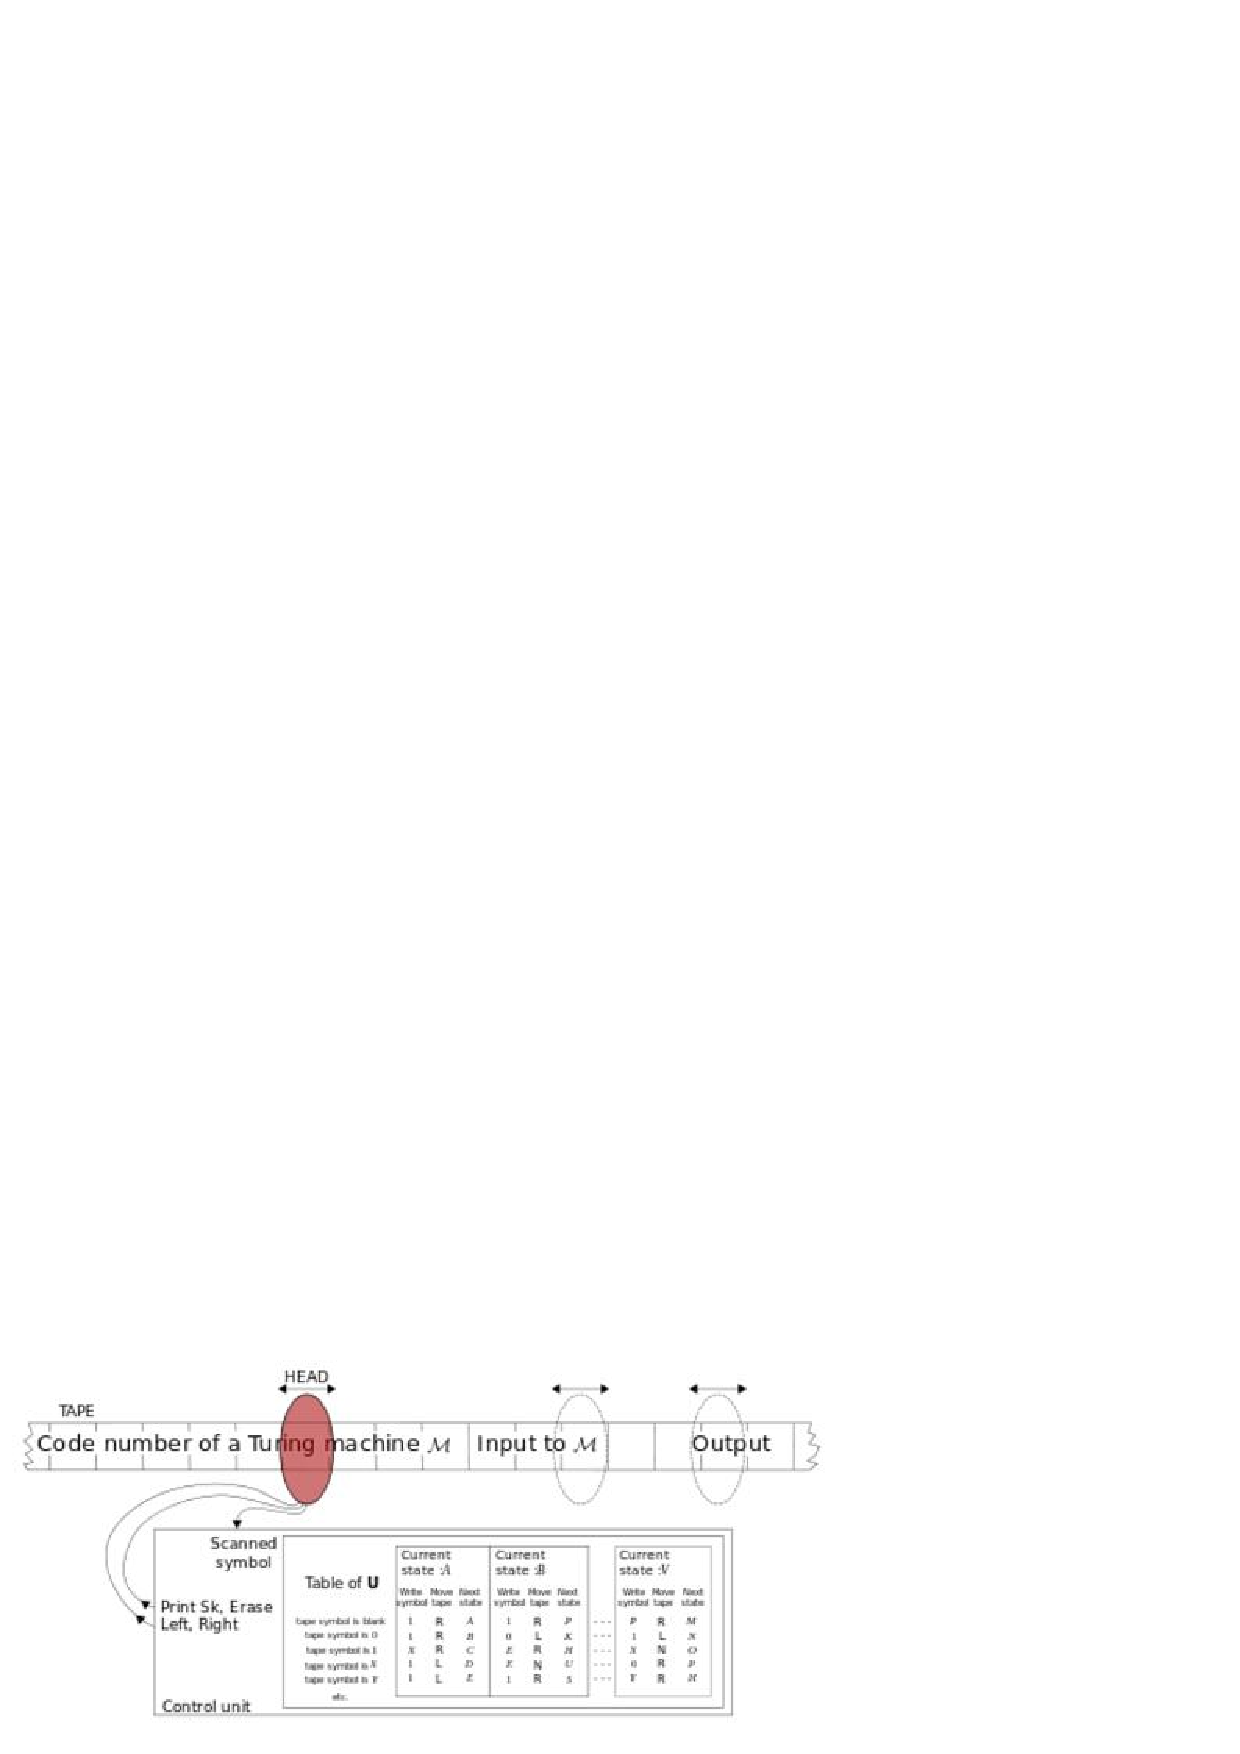
\includegraphics[width=\linewidth]{UTM.pdf}
 \caption{Universal Turing machine.}
 \label{fig:four}
\end{figure}

% \subsection{Tape Construction}
% To build the tape for a Turing machine, the universal Turing machine needs to
% store all the transition tables. In this way, all the information needed for
% computations exists. Later, for an incoming computation, we create a new tape,
% encode the input onto the tape and select a proper transition table.
% High-levelly, a ``switch'' statement over the incoming computation type is used
% to select a proper transition table at this step.
